\documentclass[12pt,titlepage]{article}
\usepackage[toc,page]{appendix}
\usepackage[linktoc=all]{hyperref}
\usepackage{listings}
\usepackage{graphicx}
\graphicspath{ {figures/} }
\usepackage{xcolor}
\usepackage{cite}
\usepackage{array}

\title{Spiking Neural Network on an FPGA}
\author{Cameron Calv, Neel Jagad, Nicholas Sica\\{\small{Advisor: Dr. Anup Das}}}
\date{November 21, 2020}

\begin{document}
\maketitle
\newpage
\clearpage
\pagenumbering{arabic}

\begin{abstract}
Individuals of every demographic may be affected by sleep apnea, an affliction causing irregular or halted breathing during periods of sleep. 
Those afflicted must obtain diagnoses by participating in polysomnography (PSG) lab tests to determine their treatment options. 
Lab tests use an array of sensors that measure quantities not limited to blood oxygen level, cardiac rhythm signals, brain electrical activity,
and eye motion \cite{elsevier}. In-lab tests offer the greatest accuracy in exchange for greater cost and the need to relocate patients from
their preferred resting environments.
Contrarily, in-home tests require less sensors, correspondingly less cost, and no need for relocation.
A disadvantage of a portable test is a reduced number of sensors measuring only blood oxygen content and most often airway pressure \cite{elsevier}.
The reduced sensor count provides fewer measurements and results in less accuracy than the in-lab tests except for the most severe of cases.
Additionally, the need to return the measuring devices has the potential to delay test results and treatment prescriptions such as a continuous
positive airway pressure (CPAP) machine.
Medical professionals and patients alike would benefit most from a solution providing the accuracy of in-lab tests at the cost and comfort of
in-home tests. 

The proposed solution that aims to reduce the gap between in-lab and in-home sleep study tests implements a spiking neural network (SNN)
machine learning model on a field-programmable gate array (FPGA). Using this SNN model, impulse-train representations of input signals
such as blood oxygen level and respiratory pressure are mapped to predictions of future apnea states and their severity.
The implementation augments the in-home sleep studies to provide real-time monitoring and levels of accuracy not normally characteristic of
portable tests. The SNN’s ability to encode time-dependent feature characteristics and to conduct asynchronous activation propagation
in addition to the FPGA’s efficiency for high-frequency switching and rapid re-programmability will facilitate low-power, high-speed operation.
As opposed to using a more general computational device, such as a graphics processing unit (GPU), the FPGA offers a smaller form factor, and
at the same time is not as permanent as application-specific integrated circuits (ASICs) which allows for rapid development. SNNs are less complex
and sparsely connected compared to related long short-term memory (LSTM) recurrent neural networks (RNNs), which makes them feasible to implement
on power- and memory-constrained devices like the FPGA. 

The project makes extensive use of open-source solutions for most of the development and makes use of a granted Xilinx FPGA board for the physical
implementation. Python is used to develop the SNN software golden model. Vivado is used to develop the hardware description of the FPGA and
generate a programmable bitstream. SymbiYosys is used for formal verification of the hardware design. Provided proprietary data as well as openly
available data from the PhysioNet Apnea-ECG Database is used for determining software accuracy and error \cite{penzel}, \cite{physiobank}. Following
hardware synthesis, a power test is conducted to determine efficiency of the implemented FPGA solution.
\end{abstract}

\tableofcontents

\listoffigures

\listoftables

\newpage
\section{Problem Description}
\subsection{Background}
Sleep apnea is a sleeping condition which causes the airway to become blocked at various times throughout the night, which is known as
obstructive sleep apnea. If the brain does not send any signals to breathe, it may be central sleep apnea. Regardless of type, it can
be very deadly to suffer from sleep apnea as it lowers the oxygen levels of the body which can reduce performance in the short-term,
and if left undiagnosed, contribute to a myriad of health issues such as a heart attack, diabetes, cancer as well as a shorter life
span \cite{hopkins}.

Sleep apnea impacts approximately 936 million people worldwide and more that are left undiagnosed due to expensive cost for diagnosis.
It is shown that sleep apnea impacts all walks of life regardless of gender, age, ethnicity, and location \cite{atsjournals}. There have
been studies performed in various regions to understand the demographic that experiences sleep apnea. To rank countries by how the many
people of the population experience sleep apnea, the apnoea-hypopnoea index (AHI) is used. The AHI is an index that essentially states
how many times a subject has experienced a severe reduction in oxygen levels which is known as an apnea episode. The criterion defined
for severity is as follows: minimal cases experience five or less episodes an hour, moderate cases experience between 15 and 30 episodes
an hour, and severe cases experience more than 30 episodes an hour. Utilizing this knowledge, the top ten countries that have an estimated
large population of people with some case of sleep apnea are the USA, France, Germany, Russia, Japan, China, Brazil, Nigeria, Pakistan,
and India. China has the largest projected population with mild cases of sleep apnea coming in at 176 million. However, this may be due to
the sheer size of the overall population. It is important to note that India also has a population size comparable to China but has projected
numbers comparable to the USA. This demonstrates that there does not seem to be any racial bias for sleep apnea. There are significant
differences in the number of men and women affected in the Americas and in European countries. These differences are negligible in Asian
countries and Australia, which may indicate a bias his could indicate that there is a bias towards men in some parts of the world
\cite{benjafield}.

To diagnose a potential candidate, a polysomnography (PSG) is taken which is a sleep study to observe the oxygen levels at various points in
the body and brain signals. However, this method is expensive, in the US it approximately costs \$2,999, and may not create a familiar sleep
environment for the candidate which may cause complications in testing that can lead to needing more sleep studies or a misdiagnosis
\cite{mdsave}. Another option is to take an in-home kit; however, this option is only for candidates that may have previous familial
history and show a higher proclivity for sleep apnea based on personal health history. The pricing of an in-home test can vary between
\$300-\$600 before insurance and can vary between \$0-\$50 after insurance \cite{rodriguez_2016}. Both solutions are deemed viable,
however, a PSG needs a technician or doctor to analyze the data in real time and to ensure that the patient has not shifted the sensors
while asleep. This same problem may be created with the in-home test kit but may result in necessary repeats of the test since it cannot
be corrected by an attending technician.

\subsection{Problem Statement}
Utilizing the data as a potential use case, the team will develop and implement a machine learning model, spiking neural network, on a
processing unit, FPGA, to improve detection and labeling of oxygen levels and brain signals.  Since a technician must be required to view
and analyze the data for sleep apnea, this model may eliminate the need for a technician until an episode has occurred or a sensor has been
shifted. This frees the technician and can perform other tasks and will simply be notified if sleep apnea has occurred or there is an adjustment
needed. In the case of the sensor being shifted for both a PSG and in-home, someone can be notified, and a mark can be indicated for such an
event and projections can be produced to reduce impact of data loss. Another contribution will be to reduce the threshold to utilize an in-home
test kit as the accuracy will be boosted since extrapolations will be made when taking in data based on previous data based on the candidate’s
preliminary analysis such as age, height, weight, and previous medical history. Utilizing the base model and tuning the meta parameters to an
individual, a model can be placed onto a CPAP machine to reduce noise pollution and energy usage. This process will hopefully bridge the gap
for SNN on FPGA implementations and produce a use case to further explore this area. 

Currently, there have been various implementations of deep learning on sleep apnea data to detect if the subject experienced sleep apnea. CNNs
and RNNs seemed to be the predominant approach. However, these methods do not process signals in real time and do not predict as the events are
occurring. A cornerstone for our implementation is to predict in near live time before an episode occurs based on the signals being read in.
One of the important features that has been leveraged previously and will be leveraged in this implementation is the oxygen saturation index
which is a measurement of oxygen in the blood. These measurements will be taken from various points of the body \cite{mostafa}.
However, most of these implementations have been on CPUs and GPUs. Another cornerstone is implementing this onto an FPGA. While there have
been implementations of FPGAs with sleep apnea in mind, there has been a larger focus on screening and monitoring strictly \cite{ashmouny}.


\section{Design Description}
\subsection{Concepts}
An FPGA is the changeable version of a CPU or GPU. It allows you to create digital logic that can be easily changed and is usually what chip makers
use to prototype a CPU or GPU before it is turned into an ASIC. A designer can take an FPGA and mold it to fit the criteria of a specific application
and therefore give speed advantages over a CPU or GPU since it is not general purpose. The downside of the FPGA is that it is very difficult to program
and changes to it require a lot more time than that of a GPU or CPU. A CPU is great for tasks that happen one after the next but suffers in tasks that
require parallelization which is where the GPU thrives. Price is a bit tricky with all the devices and will be discussed when the three are compared in
the next section.

Machine learning methods may be divided into three broad categories. Supervised learning trains a machine learning model by allowing it to categorize
a set of features into categories that have known labels. Models such as those implementing backpropagation introduce an element of correction to the
model that allows it to inch closer to what is considered a "correct" interpretation of the data. Unsupervised learning is conducted without knowledge
of a proper labeling of the data. A crucial drawback of supervised learning is the potential for the model to know the data too-well, which produces a
model that is ill-fit to generalize or adapt to new data or outliers. Supervised learning models are those that have the goal of classifying data into
a set of pre-determined categories or models that intend to fit a model to a set of data points. 

An unsupervised learning model puts the task of determining labels and feature similarities on the model, which then gives its own interpretation of how
a model should be labeled. Common labeling strategies included kernel methods that increase feature dimensionality or those that result in local or
global clustering. Unsupervised learning models have the potential of finding similarities that are too nuanced in the data, thereby missing the overall
similarities that are often sought after during exploratory data analysis.  Semi supervised learning is the midpoint between supervised and unsupervised
learning where various combinations of training and validation data are used to train a model. Models that are semi supervised usually learn upon a
training set that is developed with proper labels and then allowed to interpret unlabeled data to prevent overfitting and allow for better generalization
for data not included in training. 

Machine learning architectures other than the SNN can implement supervised, semi supervised, or unsupervised learning models. The base idea of a neural
network (NN) is that each point in a network is a unit known generally as a perceptron that aggregates a set of input signals and outputs another signal
based on some activation function of the inputs. Nodes and connections usually have biases and weights respectively that are tuned to produce a desired
output. These values are what are changed throughout a model’s learning process. Various training methods change the way the architecture learns and
process. NNs may be cyclic in nature with connections feeding back on to already visited nodes, or acyclic where no node is visited more than once.
In addition, networks may relate to various densities. Some networks connect each node of a previous layer to every node of the next layer, and some
sparse networks trim the number of connections to reduce model size and complexity. 

\subsection{Concept Evaluation}
The type of device to use could make or break the implementation of the neural network. Traditionally CPUs and GPUs were the two main choices due
to their ease of programming. GPUs were preferred over CPUs because of their highly parallelizable nature. An FPGA allows a designer to custom fit
the low-level logic to work a lot faster since it only performs one task whereas a CPU or GPU has to support a great number of instructions,
correspondingly prioritizing and scheduling them in order to be multipurpose. If a designer wants even faster speeds, they can turn to designing
an ASIC, but that causes the design to be permanent and not easily changeable. It is also significantly more difficult to design an ASIC, since more
complex logical operations require greater power, volume, and distribution considerations than a processor that splits operations into smaller, more
manageable units. Pricing of any choice of hardware has great implications for design choices. Machine learning and training has a high degree of
parallelization, therefore making CPUs generally unsuitable for precise implementations. High-end GPUs are typically in the range from \$500-\$700
while an FPGA has a price range from \$60 to \$10,000. The price usually lands around the \$3,000 mark, although it is hard to say exactly where.
FPGAs come in a variety of form factors with significant changes in memory size, programmable logic units, transistor leak and operating currents,
and many other factors. The features offered by the FPGA manufacturer will determine the final price per circuit or board. The price point may encourage
choosing the GPU over the FPGA, but GPU improvements generally cause the consumer to buy new ones sometimes on a yearly basis if the improvements are
needed. FPGAs, on the other hand, can be reprogrammed on the fly and even incorporate these improvements especially if the top of the market chip is
being used. It will be relevant and up to date significantly longer than a GPU would be.

Machine learning is a discipline that aids in automating processes through algorithmic learning and noting observations that are weighted by the
algorithm. Artificial neural networks (ANN) are a subsection of machine learning architectures, that has gained a lot of traction for being able
to process and learn about the data based on an input layer, hidden layer, and output layer and no need for a weight vector. The hidden layer is
comprised of one or many nodes that process and “judge” the data to give an output that passes to either another node or the output layer. However,
ANN’s require processing at every node within a hidden layer which requires a lot of data, can be time consuming to generate and train a model,
and have an architecture that can support and process without heavy costs. The usual complete connectivity of ANNs create great difficulty for
constrained hardware implementations since the lack of any virtually infinite memory space requires the model to be scaled down, thereby impacting
accuracy and reliability. This requires of a model scalability and efficiency that takes into consideration the limited resources present on a piece
of hardware.

Spiking neural networks (SNN) operate in a similar fashion to a brain in how to process information and decide on an action or label an object
asynchronously without needing other nodes in the hidden layer to process data. Instead of the full connectivity of a typical ANN, SNNs are more
fluid and allow for some connections to be removed, thereby reducing the need for greater memory reserves and synchronous clocking. The asynchronous
nature of an SNN incorporates a more complex temporal component to data processing that may be decoded for additional information at the network’s
output. This mode of network lends itself to less data points and generating and training time.

\subsection{Detailed Design}
While the hardware is being created, a golden model will also be designed in software. The golden model is then used to compare against the hardware and
build up a testbench to make sure the hardware works. The hardware will be built using Verilog with the SystemVerilog synthesis expansions. Verifying lower
level parts like first in first out buffers will be done using formal verification because it makes the process easier and catches difficult to spot bugs.
After simulation passes, a bitstream will be built and tests will be done to ensure the synthesis tests pass on a Virtex-7 FPGA. If any issues are found
during the synthesis tests, they will be fixed and the bitstream will be rebuilt. This last step will repeat until the synthesis tests pass.

\section{Context and Impact}
\subsection{Economic Analysis}
The anticipated impact of the FPGA SNN implementation is to bridge the gap between the high-accuracy, high-cost, in-lab PSG tests and the
low-accuracy, low-cost, in-home sleep studies. The solution must showcase greater accuracy than in-home tests at a cost lower than that of
in-lab tests. There exist four types of sleep study test with type I tests requiring the largest number of sensors, constant supervision,
and relocation, and type IV tests allowing for portability and requiring at least one sensor \cite{elsevier}. Recent estimates project that
type III tests, a single level of complexity above type IV tests, can cost on average about \$1,000.00\footnote[1]{This value was first
adjusted for November 2017 british pound conversion (1 GBP = 1.3478 USD)}\footnote{Rounded up from \$991.98 (original price was 736 GBP)},
which is more than double the price of the \$400.00\footnotemark[1]\footnote{Rounded up from \$431.30 (original price 320 GBP)} rate for
type IV tests \cite{chai}. These prices are on par with the expected rates to pay out-of-pocket for tests of these
levels. The solution must be able to use whatever signals are provided by type III or type IV tests and improve accuracy for all severities
while incurring no significant costs. 

The greatest cost incurred by the solution remains the FPGA integrated circuit that implements the SNN. The market price for different
chips can range anywhere from \$60 to a chip with a low density of logic elements to \$10,000 for a chip with hundreds of thousands of
logic elements. The most cost effective chip to buy would have to be chosen after the design is made to pick a chip that just barely fits
the design with a little bit of wiggle room. Software and formal verification utilize open-source technologies, thereby incurring no
additional price on project development. Additional costs from power consumption are minimal since the implementation respects the
constraints of a low-power, efficient solution. To prevent additional consequences from hardware integration with present type III or
type IV tests, the design uses signals already produced from test kits. This avoids the additional costs of more sensors and designates
the FPGA solution as a near plug-and-play add-on to readily available testing options.

\subsection{Environmental Impact Analysis}
Unintentional environmental effects because of the project implementation are avoided by considering the potential for lead free circuit
devices. The FPGA manufacturer, Xilinx designates that the part number XC7VX485T-2FFG1761C of project device corresponds to a RoHS 6/6
“with Exemption 15” with only enough lead content to ensure proper connection between internal die wire and package pins \cite{xilinx},
\cite{menon}.  Since the software model is configurable to various hardware constraints, compliant devices that offer further restrictions
than the device used for development continue to have the potential for drop-in replacement. 

\subsection{Social Impact Analysis}
Sleep apnea is a condition that affects all demographics without regard for socioeconomic status, and tests providing accurate and reliable
results should be made available to everyone who may be afflicted. Reducing the financial gap for in-home tests allows for quicker access
to diagnostics on sleep apnea severity and correspondingly quicker administration for treatment. Out-of-pocket expenses for in-home tests
are not billed as such unless a patient’s insurance provider preapproves the testing option and subsidizes the total cost for treatment.
Unfortunately, existing low-cost solutions may not provide the accuracy necessary for insurance coverage thereby gating the option of a
cheaper test type to those with comprehensive healthcare coverage. Augmenting existing low-cost testing kits with minimal hardware that
significantly increases prediction accuracy may lead to wider insurance approval and thereby greater accessibility for patients of all
walks of life. 

Such requirements deemed necessary for test and treatment approval depends on the type of insurance. Federal healthcare determines coverage
based on reliability and necessity standards dictated by laws on Social Security and confirmed by the U.S. Food and Drug Administration (FDA)
\cite{steinberg}. Private healthcare institutions provide coverage based on internally decided criteria. The proposed implementation addresses
such criteria, like those required by the Blue Cross and Blue Shield Association (BCBSA). The BCBSA determines coverage based on how the
experimental technology satisfies five criteria \cite{steinberg}. Technology must be approved by government authorities, backed up by scientific
evaluations, positively effective on health, at least as effective as alternative solutions, and expandable beyond its original research setting.

Accuracy tests to be delivered upon project completion address the evidence-based criteria and effectiveness-based criteria of such private
insurance solutions. Augmenting type III and type IV tests with greater accuracy provides a greater positive effect for affected populations and
increases effectiveness of already available solutions. Some tests are already portable, and the addition of the small formfactor FPGA, will not
significantly change a testing kit’s size, thereby preserving the tests portability. Following the results of both accuracy and efficiency tests,
if the solution deems to be beneficial in all regards, the potential for further approval may be explored. By aiming to satisfy various insurance
requirements, such concerns as financial availability may be addressed by the implementation allowing for greater accessibility for all social levels. 


\subsection{Ethical Analysis}
Reliability is the greatest concern, as its absence reduces all faith in the project’s design. The implementation must ensure high accuracy,
minimize false negatives, and minimize false positives. High accuracy results from the proper configuration of the software golden model and the
accurate implementation of the model and training rules on the FPGA. Multiple verification tests quantify the accuracy of the implementation by
reporting minimized error metrics such as least mean squares (LMS) error and mean squared error (MSE). A false positive reading corresponds to the
implementation incorrectly determining the severity of sleep apnea to be more severe than is correctly determined. False positive readings by the
model are to be avoided because any falsities decrease the viability of the solution and may indicate inconsistent results. A false negative
reading corresponds to the implementation incorrectly determining the severity of sleep apnea to be less severe than is correctly determined.
False negative readings may detriment an individual by providing proof for a treatment that insufficiently mitigates the sleep apnea affliction.
In some cases, these types of decisions may lead to insufficient enough treatment as to have irreversible, detrimental effects on the patient.
Since a low level of reliability may lead to permanent harm of an otherwise healthy individual, the absolute minimization of all false readings
is pursued. 

\section{Approach}
\subsection{CAD/CAM}
\subsection{Animations}
\subsection{Simulations}
\subsection{Numerical Modeling}

\section{Materials/Resources}
\subsection{Hardware}
\begin{itemize}
	\item Xilinx FPGA
	\item Verilog: Language used to write the hardware for the FPGA
	\item Xilinx Vivado: Used for programming the FPGA
	\item SybiYosys: Used for formal verification of the hardware subsystems
\end{itemize}
\subsection{Software}


\section{Project Management}
\subsection{Team Organization}
All team members are responsible for the tasks they have volunteered for. Team members choices correspond to the strengths and focus areas that they study.
Member Cameron Calv who majors in electrical engineering and computer engineering focuses on the formal verification of hardware, software development of
the testbench, and the implementation efficiency analysis. Member Neel Jagad who majors in computer engineering leads software design implementing the SNN
golden model and conducting experimental data analysis and feature selection. Member Nick Sica who majors in computer engineering and minors in computer
science leads hardware designing performing the development of the hardware Verilog for the FPGA, synthesizing the programmable bitstream, and assisting in
final analysis and verification. The faculty member advising the team is Dr. Anup Das. 

Group tasks will be assigned using a Kanban project management board allowing for accurate planning of deadlines and compartmentalization of responsibilities.
Code flow including that for software models and hardware descriptions is facilitated using Git version control and code storage on GitHub. 

\subsection{Schedule and Milestones}
Project progress is conducted in a six-month time frame split up into three academic terms as shown in the gantt chart in Table~\ref{tbl:gantt}.
Dark colorings represent portions of time where the task is being worked on with shading under assignments corresponding to the participation of
the corresponding team member. The initial month of progress determines familiarity with sleep
apnea datasets and obtaining access authorization for proprietary data once familiarity is established. Following the feature selection from available data
the software golden model of the SNN is developed as well as the initial architecture layout on the FPGA. Much of the winter season is spent on configuring
the model and developing the hardware framework. Connection between the hardware and software will be facilitated with a software testbench. Following the
connection of the hardware and the software, prediction accuracy tests will be conducted to determine how, if at all, the model needs to be tuned. Concluding
progress are the final efficiency tests for the FPGA implementing the SNN following the synthesis of the hardware bitstream. The following chart showing the
time dedicated to each design goal and the relative participation of each team member to the goal is provided below.

\subsection{Project Budget}
The total cost of all materials consists only of the expenses incurred by the hardware design choice. The FPGA provided by Xilinx is the only part that
incurs a cost because while there is a licensing fee of \$3,500 for Vivado, there is a free webpack or lab version that can be used to program the FPGA.
All other technologies used are open-source or publicly licensed databases.

\subsection{Success Benchmarks}
Performance metrics such as the MSE and LSM error will give accuracy results from the software and hardware implemented model. Efficiency tests run on the
hardware give a method of quantifying the total energy cost of the implementation which must remain as low as possible. 

\bibliographystyle{IEEEtran}
\bibliography{ref}

\begin{appendices}
\section{Detailed Project Management}
\begin{table}[!htb]
	\caption{Gantt chart showing the responsibilities of each team member}
	\label{tbl:gantt}
	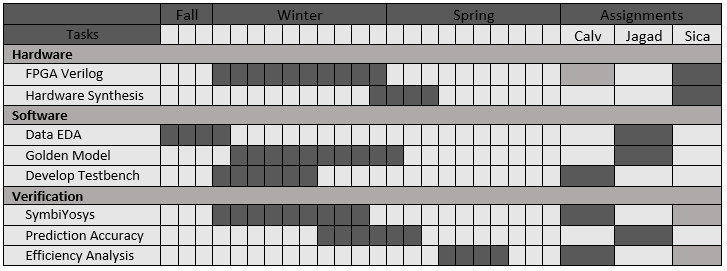
\includegraphics[width=\linewidth]{gantt.png}
\end{table}
%\section{Programming Source Code and Drawings}
\section{Teamwork Contract}
\end{appendices}

\end{document}

%\begin{figure}[!htb]
%  \centering
%  \includegraphics[width=4in]{}
%  \caption{}\label{fig:}
%\end{figure}

%%% Local Variables:
%%% mode: latex
%%% TeX-master: t
%%% End:
